\documentclass[tikz,border=2pt]{standalone}
\usepackage{amsmath,amssymb}
\usepackage{pgfplots}
\pgfplotsset{compat=1.18}

\begin{document}
% CDF and survivor function of an Exp(1) variable: at every x the two values add up to 1.
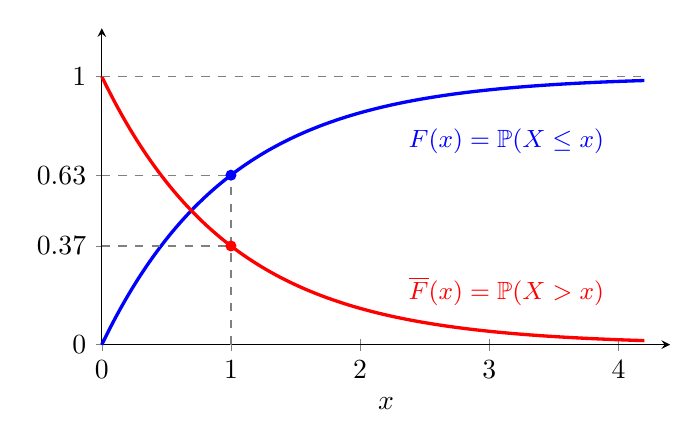
\begin{tikzpicture}
	\begin{axis}[
		axis lines=left, xmin=0, xmax=4.4, ymin=0, ymax=1.18,
		xtick={0,1,2,3,4}, ytick={0,0.368,0.632,1}, yticklabels={$0$,$0.37$,$0.63$,$1$},
		xlabel={$x$},
		samples=120, smooth, width=8.8cm, height=5.6cm, clip=false
		]
		\addplot[blue, very thick, domain=0:4.2] {1-exp(-x)};
		\addplot[red, very thick, domain=0:4.2] {exp(-x)};
		\draw[gray, dashed] (axis cs:0,1) -- (axis cs:4.2,1);
		\draw[gray, dashed] (axis cs:1,0) -- (axis cs:1,0.632);
		\draw[gray, dashed] (axis cs:0,0.368) -- (axis cs:1,0.368);
		\draw[gray, dashed] (axis cs:0,0.632) -- (axis cs:1,0.632);
		\fill[blue] (axis cs:1,0.632) circle (2pt);
		\fill[red] (axis cs:1,0.368) circle (2pt);
		\node[blue, anchor=north west, font=\small] at (axis cs:2.3,0.84) {$F(x)=\mathbb{P}(X\le x)$};
		\node[red, anchor=south west, font=\small] at (axis cs:2.3,0.11) {$\overline F(x)=\mathbb{P}(X>x)$};
	\end{axis}
	
\end{tikzpicture}
\end{document}
